\documentclass[12pt]{zettel}

\usepackage{multicol}

%\renewcommand{\gregor}{\put(10.0,-3.5){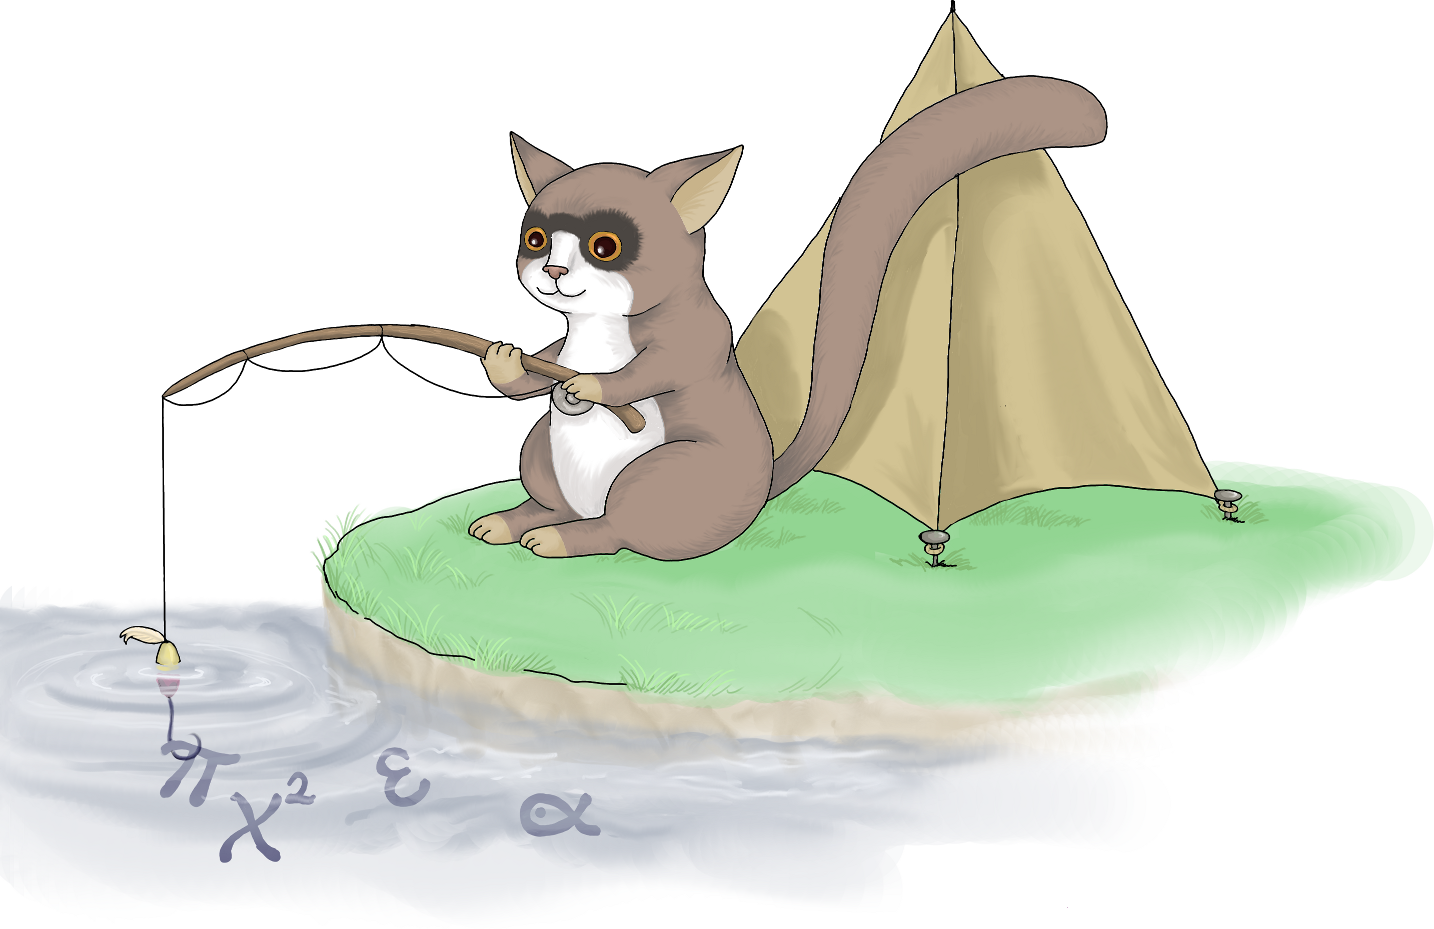
\includegraphics[scale=0.18]{campgregor}}}

\usepackage{framed}
\definecolor{shadecolor}{rgb}{.97,.97,.97}

\geometry{tmargin=1.5cm,bmargin=1.5cm,lmargin=2.9cm,rmargin=2.9cm}

\renewcommand{\gregor}{\put(9.2,-3.5){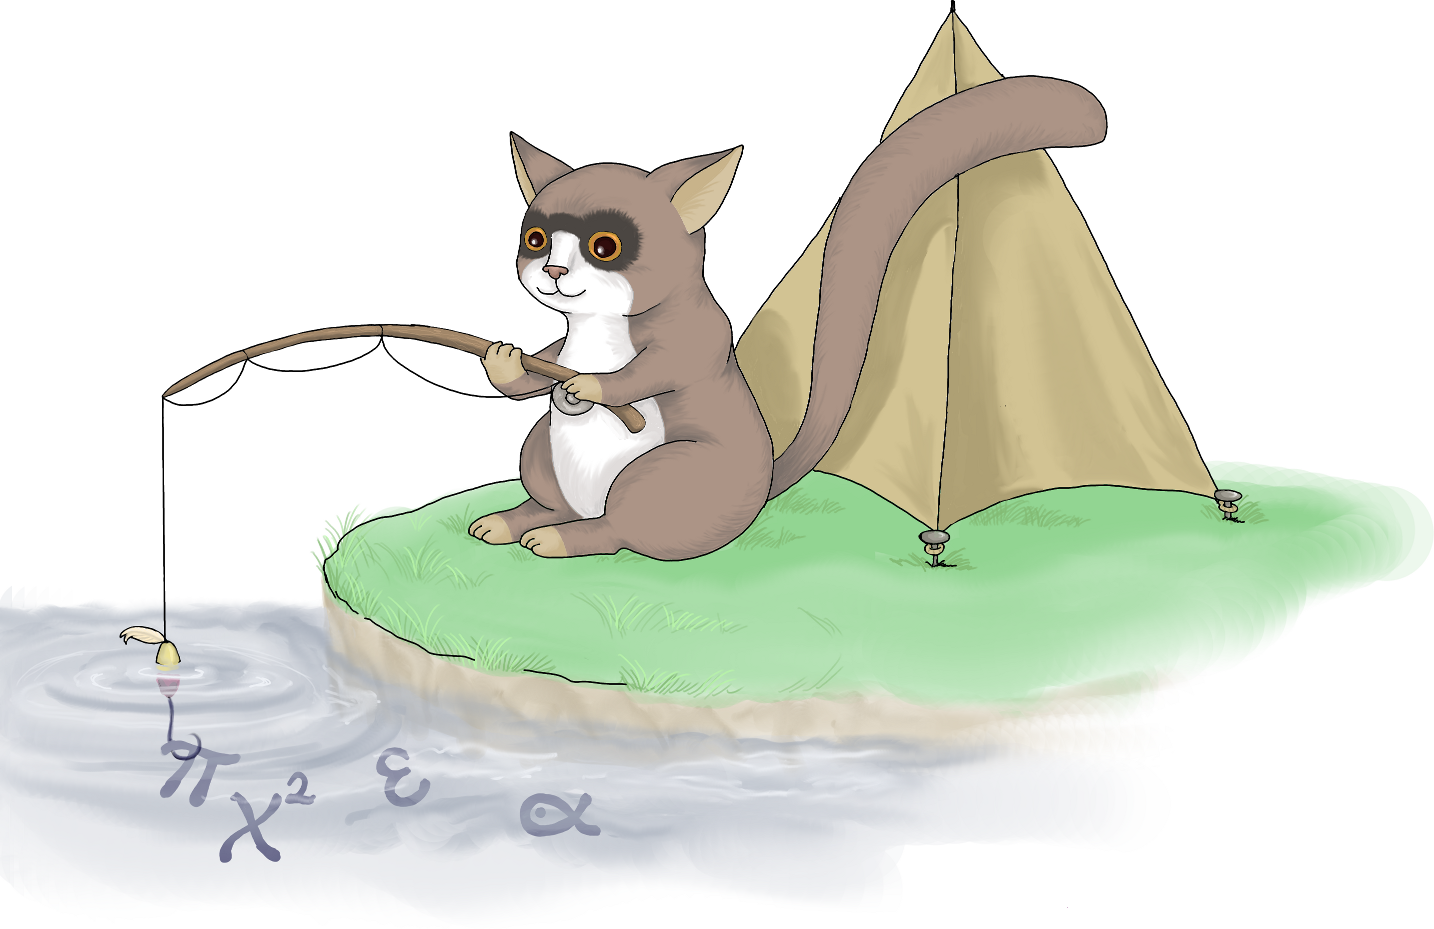
\includegraphics[scale=0.16]{campgregor}}}

\def\chopline#1;#2;#3;#4;#5 \\{
  \def\vorname{#2}
  \def\nachname{#1}
\def\mann{#3}
\def\strasse{#4}
\def\plzort{#5}
 }

\newif\ifmore\moretrue

\begin{document}

\newread\quelle
 \openin\quelle=alles.csv
 
 \loop
  \read\quelle to \zeile
  \ifeof\quelle
   \global\morefalse
  \else
   \expandafter\chopline\zeile\\

\renewcommand{\anschrift}{
      \vorname~\nachname \\
      \strasse \\
      \plzort
			}
\renewcommand{\datum}{\today}
\renewcommand{\betreff}{Mathecamp des Matheschülerzirkels Augsburg}

\makeletterhead{}
\vspace{-2em}

\mann~\vorname,

wir freuen uns sehr, dass du mit uns aufs Mathecamp
fährst. Unten stehen die wichtigsten Informationen für dich und deine Eltern.

%Wir bedanken uns herzlich bei \emph{Bündnis für Augsburg}, dem
%\emph{Mathematisch-Physikalischen Verein} und den Professorinnen und
%Professoren der Lehrstühle für \emph{Algebra und Zahlentheorie},
%\emph{Angewandte Analysis} und \emph{Nichtlineare Analysis} des Instituts für
%Mathematik für ihre Unterstützung.

%Besonderer Dank gebührt einem Professor des
%Lehrstuhls für \emph{Analysis und Geometrie}, ohne dessen engagierten Einsatz
%das Mathecamp nicht denkbar gewesen wäre.

%Ferner bedanken wir uns bei Ihnen, liebe Eltern, für die zahlreichen
%Spenden.

Wir sehen uns am 16. August! Wenn du in der Zwischenzeit Fragen hast, zögere
nicht, uns anzuschreiben oder anzurufen.

\vspace{1em}

Dein Team vom Mathezirkel

\vspace{1em}

%{\small Meru Alagalingam, Martin Baur, Ingo Blechschmidt, Tim Dafler, Philipp Düren,
%Alexander Engel, Kathrin Helmsauer, Christian Hübschmann, Jil Hümmer, Sven Prüfer,
%Lisa Reischmann, Peter Uebele}

%{\small Meru Alagalingam, Tim Baumann, Martin Baur, Ingo Blechschmidt, Tim
%Dafler, Philipp Düren, Alexander Engel, Johanna Fleckenstein, Kathrin
%Helmsauer, Prof. Dr. Marco Hien, Christian Hübschmann, Jil Hümmer, Simon
%Kapfer, Sven Prüfer, PD Dr. Peter Quast, Lisa Reischmann, Peter Uebele, Prof.
%Dr. Timo Schürg, Carina Willbold, Christopher Wulff, Stephanie Zapf}

\begin{shaded}
\textbf{Anreise per Bus.} Falls du auf der Anmeldung angegeben hast, dass du mit dem
Mathezirkelbus nach Violau fahren möchtest, komm bitte am 16. August um
9:30 Uhr zum Messeparkplatz bei der Uni Augsburg: Universitätsstr. 16, 86159
Augsburg. Karte: \url{https://goo.gl/maps/h4lBY}

\textbf{Individuelle Anreise.} Falls du nicht mit uns im Bus nach Violau fährst, komme bitte
zwischen 10:00 Uhr und 11:00 Uhr direkt zum Bruder-Klaus-Heim (außer deine Eltern haben etwas anderes mit uns ausgemacht):
St. Michael Straße 15, 86450 Violau-Altenmünster. Anfahrt:
\url{http://tiny.cc/3lxrjx}
\end{shaded}

\begin{shaded}
\textbf{Rückreise per Bus.} Wir kommen am 20. August um 17:30 Uhr am Messeparkplatz an der Universität Augsburg an der Stelle, wo wir abgefahren sind, an. Von dort können dich deine Eltern abholen.

\textbf{Individuelle Rückreise.} Wenn dich deine Eltern direkt in Violau abholen, ist das zwischen 16:30 Uhr und 17:30 Uhr möglich, oder sonst wie von deinen Eltern mit uns abgesprochen.

Wenn du und deine Eltern euch nicht mehr sicher seid, was ihr bei der Anmeldung angegeben habt,
schickt uns einfach eine kurze Mail oder ruft an.
\end{shaded}

%\newpage

\begin{shaded}
\textbf{Kontakt.} Für Fragen stehen wir euch jederzeit zur Verfügung.
\begin{tabbing}
  Während des Camps:\quad \= \kill
  Vor dem Camp: \> Tel.: 0821/598-5601, 0821/598-5805 \\
  \> Mail: \texttt{mathezirkel@math.uni-augsburg.de} \\[0.5em]
  Während des Camps: \> Handy: 0163/7363229, 0176/81160586, 0179/2129137 \\
  \> Festnetz des Bruder-Klaus-Heims: 08295/1097 \\
  \> Fax: 08295/499
\end{tabbing}
\vspace{-1em}
\end{shaded}

\newpage

\begin{shaded}
\textbf{Packliste.} Bitte bring unbedingt folgende Dinge mit:
%\begin{multicols}{2}
\begin{itemize}
\item \textbf{Einzunehmende Medikamente}
\item \textbf{Krankenkassenkarte}
\item \textbf{Kleidung} (auch für Freizeit/Sport)
\item \textbf{Kulturbeutel}
\item \textbf{Handtuch}
\item \textbf{Bettwäsche} (oder 5 EUR)
\item Mäppchen mit Stiften, Geodreieck und Radierer %(ein Taschenrechner ist
%nicht nötig)
\item Büchlein, Heft oder Hefter zum Mitschreiben und Abheften
\item Sportschuhe für draußen und Hallenschuhe
\item Hausschuhe
\end{itemize}
%\end{multicols}
Gerne kannst du auch mitnehmen:
%\begin{multicols}{2}
\begin{itemize}
\item Taschenlampe
\item Handy zum Kontaktieren deiner Eltern
\item Schwimmsachen
\item Bücher
\item Dein Lieblings-(Brett-)Spiel
\item Handliches Musikinstrument
\item Süßigkeiten, Kekse, Knabberzeug (aber nicht übertreiben, für Essen
ist gesorgt)
%\item Geld für Getränke
\end{itemize}
%\end{multicols}
Auch ohne viele elektronische Geräte wird dir auf jeden Fall nicht langweilig werden.
Alkohol, Messer und Ähnliches darfst du nicht mitbringen. 

%Bei schwerwiegenden Verstößen müssen wir uns leider vorbehalten, dich gegebenenfalls eher abholen zu lassen.
\end{shaded}

\vfill

\begin{center}
  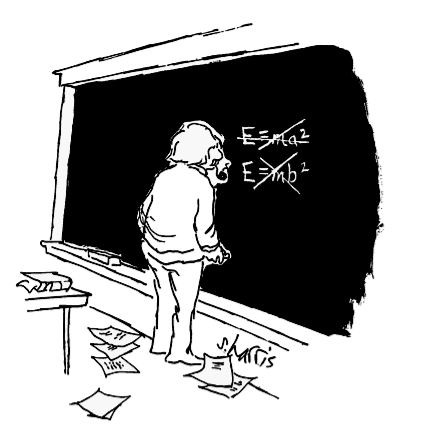
\includegraphics[scale=0.4]{einstein}

  \emph{Es ist nicht so, dass ich besonders klug wäre, ich bleibe einfach
  hartnäckig daran, \\ bis ich das Problem gelöst habe.}

%It's not that I'm so smart, it's just that I stay with problems
%  longer.}
  -- Albert Einstein
\end{center}

\newpage

\fi
\ifmore\repeat

\closein\quelle

\end{document}
